
%%%%%%%%%%%%%%%%%%%%%%% paper_sem_web.tex %%%%%%%%%%%%%%%%%%%%%%%%%
%
% This is the LaTeX source for the instructions to authors using
% the LaTeX document class 'llncs.cls' for contributions to
% the Lecture Notes in Computer Sciences series.
% http://www.springer.com/lncs       Springer Heidelberg 2006/05/04
%
% It may be used as a template for your own input - copy it
% to a new file with a new name and use it as the basis
% for your article.
%
% NB: the document class 'llncs' has its own and detailed documentation, see
% ftp://ftp.springer.de/data/pubftp/pub/tex/latex/llncs/latex2e/llncsdoc.pdf
%
%%%%%%%%%%%%%%%%%%%%%%%%%%%%%%%%%%%%%%%%%%%%%%%%%%%%%%%%%%%%%%%%%%%


\documentclass[runningheads,a4paper]{llncs}
\usepackage[utf8x]{inputenc}
\usepackage{amssymb}
\setcounter{tocdepth}{3}
\usepackage{graphicx}

\usepackage{url}
\urldef{\mailsa}\path|{manuel.b.dudda, robert.c.brylka, frank.b.reichwein,}@student.hs-rm.de|    
\newcommand{\keywords}[1]{\par\addvspace\baselineskip
\noindent\keywordname\enspace\ignorespaces#1}

\begin{document}

\mainmatter  % start of an individual contribution

% first the title is needed
\title{Semantic Web Technologien:\\FIFA's Fu\ss ball-Weltmeisterschaft 2014 in Brasilien bekommt eine semantische Unterst\"utzung.}

% a short form should be given in case it is too long for the running head
\titlerunning{Semantic Web: Brasil WM 2014}

% the name(s) of the author(s) follow(s) next
%
% NB: Chinese authors should write their first names(s) in front of
% their surnames. This ensures that the names appear correctly in
% the running heads and the author index.
%
\author{Manuel Dudda%
\thanks{Herzlichen Dank, dass Du das Projekt im allein Gang auf die Beine gestellt hast und von uns nur verlangt hast, dass wir einmal die Hose runter lassen :-).}%
\and Robert Brylka\and Frank Reichwein}
%
\authorrunning{Brasil WM 2014 mit Semantic Web}
% (feature abused for this document to repeat the title also on left hand pages)

% the affiliations are given next; don't give your e-mail address
% unless you accept that it will be published
\institute{Hochschule RheinMain Informatik Master of Science \\
Fachbereich Design Informatik Medien \\
Campus Unter den Eichen 5
65195 Wiesbaden , Deutschland\\
\mailsa\\
\url{http://www.http://semanticwc.herokuapp.com}}

%
% NB: a more complex sample for affiliations and the mapping to the
% corresponding authors can be found in the file "llncs.dem"
% (search for the string "\mainmatter" where a contribution starts).
% "llncs.dem" accompanies the document class "llncs.cls".
%

\toctitle{Lecture Notes in Computer Science}
\tocauthor{Authors' Instructions}
\maketitle


\begin{abstract}
Große Sportereignisse haben schon immer große Menschenmaßen begeistert. So auch die Events die die Disziplin Fußball betreffen. Dieses Paper beschreibt ein Projekt, das sich als Ziel die Vorstellung der Ereignisse der diesjährigen Fußballweltmeisterschaft gesetzt hat. Der Fokus dieser Anwendung liegt auf der Aktualität der präsentierten Daten sowie einer auf die Mobilen-Endgeräte angepassten Repräsentation. Für die Vielfalt der präsentierten Daten sowie deren Richtigkeit sorgte eine Informationssynthese aus mehreren Quellen. Um die Informationen weitestgehend für automatische Weiterverarbeitung vorzubereiten wurden alle Daten um semantische Bedeutung aus gängigen Sport-Ontologien ergänzt.
\end{abstract}

\section{Introduction}

\section{Related Work}

Bei der Recherche in dem Bereich der Fußbaleregnisse mit semantischen Hintergrund hat sich unsere Aufmerksamkeit auf drei Quellen gerichtet, die Sport-Ontologie\footnote{\url{http://www.bbc.co.uk/ontologies/sport}} der BBC, die Soccer Voc Ontologie\footnote{\url{http://purl.org/hpi/soccer-voc/}} des Hasso-Plattner-Institut sowie der World Cup\footnote{\url{http://www.http://worldcup.sfg.io/}} JSON API.\\ Die Future Media and Technologie Abteilung der BBC setzt semantische Technologien um die intern relevanten Inhalte automatisch verwalten zu können. Der erste große Einsatz der semantischen Technologien war die Gestaltung der Internetseite\footnote{\url{http://news.bbc.co.uk/sport2/hi/football/world_cup_2010/default.stm}} mit Informationen zu dem FIFA World Cup 2010. Die dabei eingesetzte Ontologie ist seither frei zugänglich. \\
Die Arbeitsgruppe "Semantic Technologies"\footnote{\url{http://hpi.de/meinel/knowledge_tech/semantics.html}} an dem Hasso-Plattner-Institut im Potsdam veröffentlichte 2012 ein Paper zu Linked Soccer Data\cite{url_lsd}. Im Rahmen dieses Papers wurde ein Datensatz mit Fußballinformationen vorgestellt, der mit der LOD Cloud\footnote{\url{http://linkeddata.org/}} verknüpft wurde. Die dabei verwendete Ontologie kann frei verwendet werden und stellt eine gute Ergänzung der Sport-Ontologie der BBC dar.\\
Bei der World Cup API handelt sich um ein von Eric Stiens\footnote{\url{http://softwareforgood.com/soccer-good/}} betreutes Projekt. Dessen Ziel ist es die aktuellen Fußballereignisse für jeden frei verfügbar zu machen. Neben der frei verfügbaren Informationen, die als JSON Dateien vorliegen, ist auch die API selbst für Weiterentwicklung als Projekt\footnote{\url{https://github.com/estiens/world_cup_json/}} auf Github freigegeben. 

\newpage
\section{Bestimmung der Informationsquellen}\label{infoQuell}

Die Fußballweltmeisterschaft ist allgemein ein belebtes Thema in der digitalen Welt. Um geeignete Quellen für die gesuchte Informationen zu finden wurde eine tiefgründige Recherche durchgeführt. Die unten aufgeführte Tabelle zeigt ein Ausschnitt aus der Zusammenstellung in der die geeigneten Quellen aufgeführt wurden. Wie man an der Zusammenstellung erkennen kann verfügen nicht alle Quellen über die gleiche Informationsfülle. Dabei ist die Open Football \cite{url_openfootball} Datenbank aufgrund der nicht aktuellen Informationen für weitere Verwendung uninteressant. Die Football Data \cite{url_footballdata} sowie die World Cup \cite{url_worldcup} Datenbank zeigen beide eine sehr gute Fülle an brauchbaren Informationen. Bei einer weiteren Recherche zu der Word Cup Datenbank wurde die offengelegte API gefunden die einen direkten Zugriff auf die offizielle Seite der FIFA ermöglicht. Wie die letzte Spalte der Zusammenstellung zu entnehmen ist, ist die offizielle Seite des Internationalen Fußballverbandes die beste Informationsquelle. 
Daraus resultierend wurde ein Fork der Soccer for good API erstellt und dieser unseren Bedürfnissen angepasst. Durch die Anpassungen wurde die API um Informationen zu den Spielern, Trainern und Schiedsrichtern erweitert. Es wurden damit alle für die Anwendung relevaten Informationen in die API integriert. Dieser Fork Cup bietet bietet entsprechende REST\footnote{\textbf{Re}presentational \textbf{S}tate \textbf{T}ransfer} Endpunkte an. Die Rückgabe dieses Services ist eine JSON\footnote{\textbf{J}ava\textbf{S}cript \textbf{O}bject \textbf{N}otation} Datei mit allen relevanten Informationen. 

\begin{center}
%\begin{table}

\begin{tabular}{|l|c|c|c|c|c|}   \hline 
 & Football Data 	& Open Football 	& Footbal DB  &	World Cup  & FIFA  \\ \hline
References & \cite{url_footballdata} & \cite{url_openfootball} &  \cite{url_footballdb} &
 \cite{url_worldcup} & \cite{url_fifa} \\ \hline
 
Teams				& + & + & +	& + & +		\\ \hline
Gruppen				& - & + & -	& + & +		\\ \hline
Spiele				& + & + & -	& + & +		\\ \hline
Stadien				& + & + & -	& + & +		\\ \hline
Uhrzeiten			& + & + & -	& + & +		\\ \hline
Spieler				& + & + & - & - & +		\\ \hline
Spielergebnisse		& + & + & + & + & + 		\\ \hline
Torschützen/min		& +/+ & 	+/+ & - & + & +/+ 	\\ \hline
Schiedsrichter		& - & - & - & - & +		\\ \hline
Trainer				& - & - & - & - & +		\\ \hline
Spieltag 			& + & + & + & + & +		\\ \hline
Aktuell				& - & - & + & + & +  \\ \hline
Besucherzahl			& + & - & - & - & +		\\ \hline
			 
\end{tabular}
%\end{table}

%\label{tab:tab1} 

%\caption{Zusammenstellung der wichtigsten Informationsquellen}	
\end{center}


Eine wichtige Rolle bei der Wahl der API hat letztendlich auch der Finanzielleraspekt gespielt. Es gibt eine ganze Reihe an gut organisierten und stets aktuellen Datenbanken, die jedoch eine monatliche Gebühr mit sich tragen. Für dieses Projekt wurde jedoch eine Vereinbarung getroffen, rein Quelloffene Lösungen zu verwenden. Dadurch sind Finanziellabhängige Projekte direkt bei der Recherche ausgeschlossen worden. 
  
\newpage
\section{Ontologien}




Die Abbildung \ref{fig:example} zeigt einem Graphen, der für einem exemplarischen Ausschnitt aus der mit dem Ontologien vorbereiteten Daten, aufgebaut wurde. An diesem Beispiel ist die Verflechtung der beiden Ontologien sehr gut sichtbar.

\begin{figure}
\centering
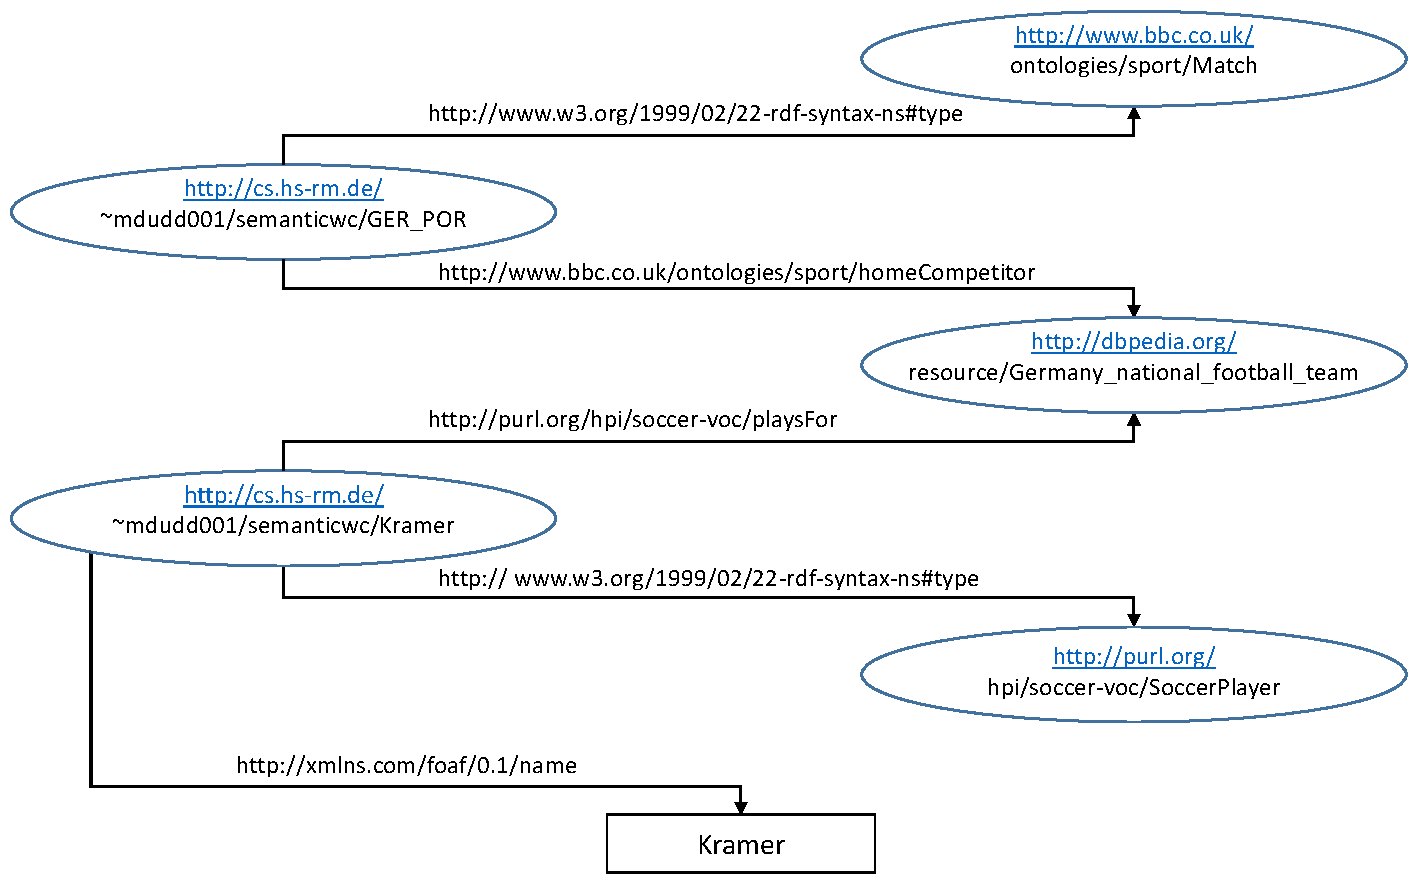
\includegraphics[height=7.2cm]{graph_manus}
\caption{Exemplarische Ausschnitt aus der RDF.}
\label{fig:example}
\end{figure}

\newpage
\section{Application // Implemetierung}


Bei der Wahl des Framework für diese Anwendung fiel die Entscheidung zu Gunsten von Ruby on Rails \footnote{http://www.rubyonrails.org/}. Dieses quelloffenes Web Application Framework bietet sehr gute Unterstützung bei Entwicklung von Semantik Web Applikationen um die RDF Datenbank oder den SPARQL Client zu nennen. Für Gestaltung der Seiten sowie als Unterstützung für die Mobilen-Endgeräte, z.B. für den Swipe-Efect,  wurde die jQuery mobile\footnote{http://www.jquerymobile.com/} Bibliothek eingesetzt. 

Die Abbildung \ref{fig:example} zeigt eine Übersicht über den Technick-stack. Um die Daten aus der FIFA Seite zu beziehen wurde ein REST Server aufgestellt der auch separat über \texttt{sfgapi.herokuapp.com} abrufbar ist. Die so vorbereiteten Daten werden folglich mit den zuvor beschriebenen Ontologien aufbereitet. Da die Anwendung sich zunächst auf ein Sportliches Ereignis beschränkt, in diesem Fall die Fußballweltmeisterschaft, wurde hierfür keine zusätzliche Datenbank angelegt. Stattdessen werden alle Datensätze als RDF-Trippel in einer Datei gespeichert.
\begin{figure}
\centering
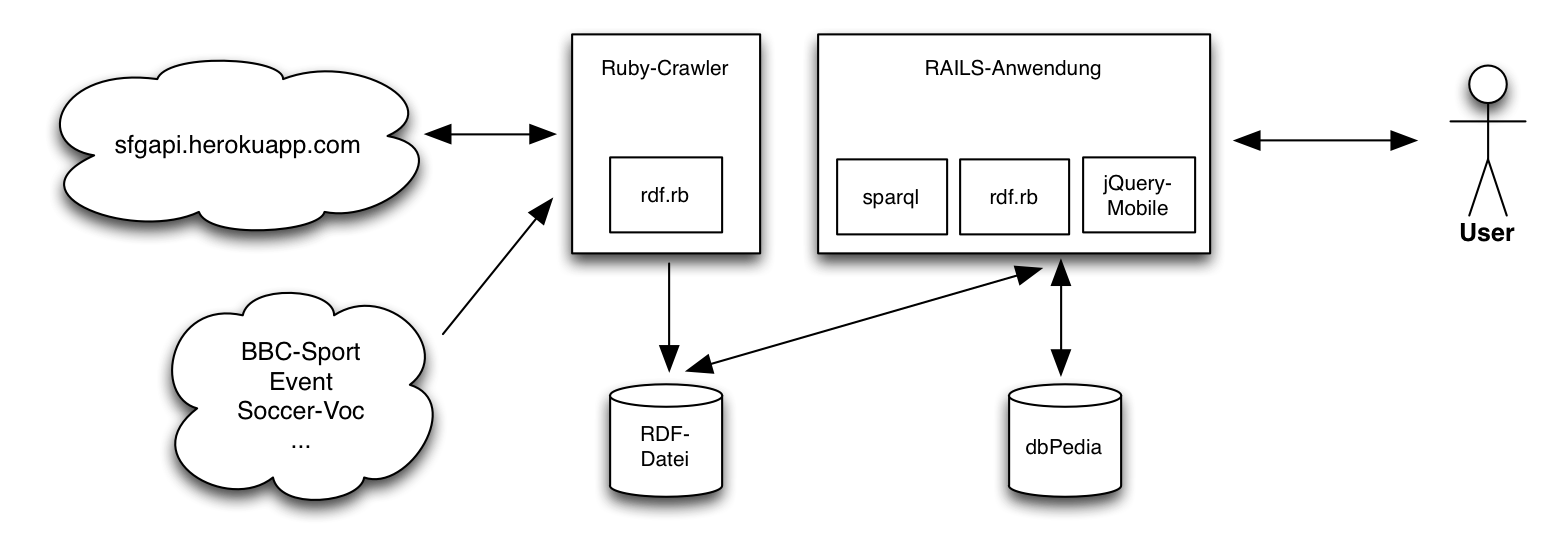
\includegraphics[height=4.2cm]{technik-stack}
\caption{Technik-stack.}
\label{fig:example}
\end{figure}


Als Abfragesprache für die so vorbereiteten Informationen wurde SPARQL ausgewählt. Neben der RDF-Datei, die als primäre Endpoint fungiert, wird für zusätzliche Informationen die DBpedia als sekundäre Endpoint eingesetzt. 

\newpage
Die Abbildung \ref{fig:screenshots} zeigt drei Screenshots der fertigen Anwendung. Oben links ist die Startseite zu sehen, auf der immer der aktuelle Spieltag anzeigt wird. Links unten ist ein Ausschnitt aus der Ansich die Informationen zu dem Stadien präsentiert. Die Rechtehälfte des Screenshots zeigt wiederum eine Ansicht die die Informationen zu einem Trainer einer Mannschaft präsentiert. Da die Anwendung vorwiegend auf Mobile-Endgeräte ausgelegt ist, wurde bei der Gestaltung der einzelnen Ansichten ein große Wert auf die Übersichtlichkeit gelegt. Für eine schnelle Navigation wurden zudem zwei Buttons eingepflegt. Der 'Home' Button, der in jeder Ansicht in der oberen linke Ecke zu sehen ist, führt immer zu der Seite mit den aktuellen Spieltag. Mit dem 'Bar' Button, in oberen rechten Ecke jeder Ansicht, kann eine Seitenansicht mit mehreren Filteroptionen eingeblendet werden. Dabei kann der Inhalt nach dem Team, der Gruppe, dem austragenden Stadion oder dem Spieltag sortiert werden.

       
\begin{figure}
\centering
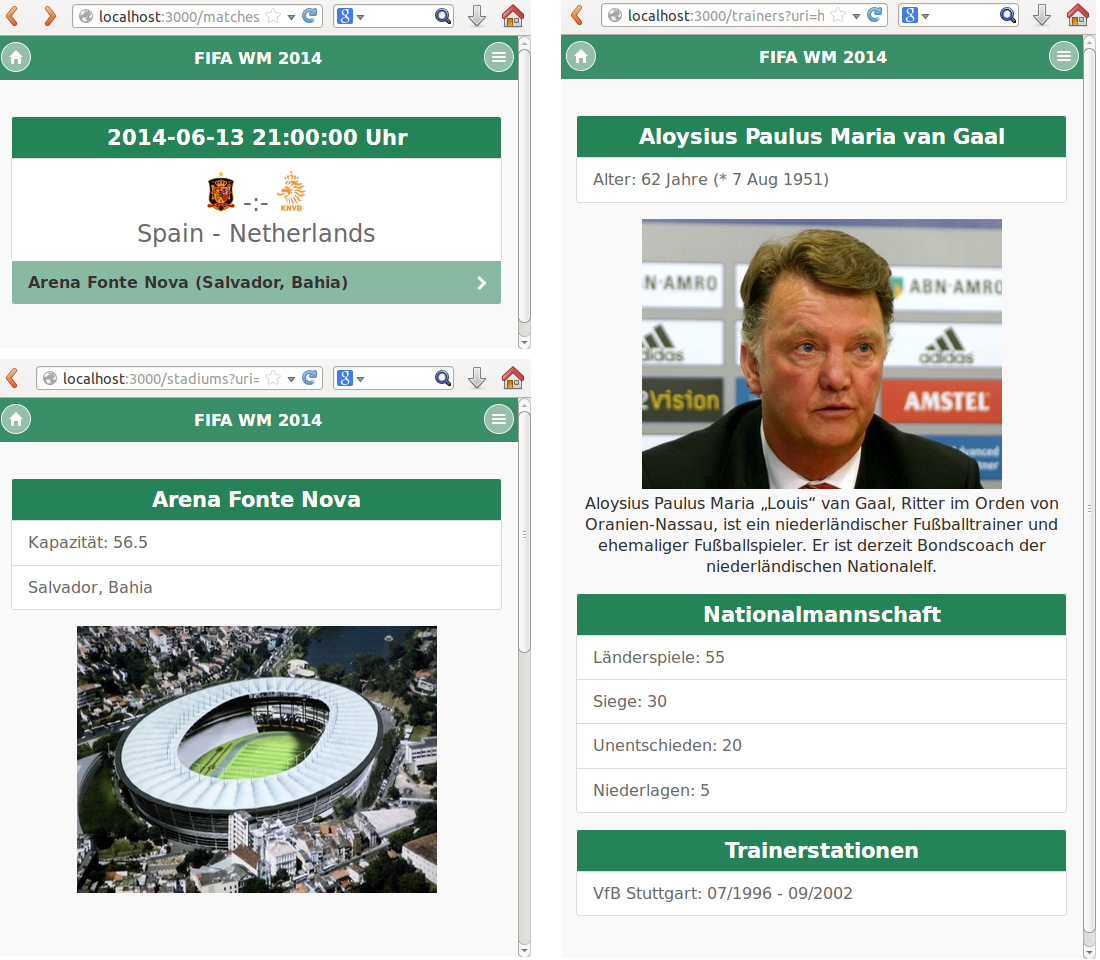
\includegraphics[height=8.2cm]{screenshots}
\caption{Screenshots der Anwendung.}
\label{fig:screenshots}
\end{figure}

\newpage

\section{Zusammenfassung und Ausblick}

Im Rahmen dieses Projekts wurde eine Anwendung entwickelt, die alle wichtigen Informationen, zu der 2014 in Brasilien stattfindenden Fußball Weltmeisterschaft, bereithält. Als Informationsquelle dient hierbei die offizielle FIFA Webseite, die mit Daten aus der DPpedia ergänzt wurde. Die semantische Aufbereitung wurde mit Hilfe der BBC Sport sowie der Socker Voc Ontologie gestaltet.  

Unsere Anwendung bietet eine solide Grundlage für Weiterentwicklungen die nicht nur den Bereich Fußball betreffen. Bezogen auf die Fußballereignisse kann eine leichte Portierung auf die nächste Weltmeisterschaft oder Europameisterschaft stattfinden. Denkbar ist aber auch eine Abwandlung zur Informationspräsentation der Spiele der Bundesliga Mannschaften. 



\begin{thebibliography}{4}

\bibitem{url_lsd}Linked Soccer Data,
Tanja Bergmann, Stefan Bunk, Johannes Eschrig, Christian Hentschel, Magnus Knuth, Harald Sack, and Ricarda Schüler\\
Hasso Plattner Institute for Software Systems Engineering, Potsdam, Germany\\
Letzter Zugriff: 22. Juni 2014\\
\url{http://ceur-ws.org/Vol-1026/paper6.pdf}

\bibitem{url_bbc}BBC ONTOLOGIES,
Letzter Zugriff: 26. Juni 2014\\
\url{http://www.bbc.co.uk/ontologies}

\bibitem{url_jquery}jQuery mobile,
Letzter Zugriff: 26. Mai 2014\\
\url{https://demos.jquerymobile.com/1.4.2/}

\bibitem{url_smm}Semantic Media Mining,
Letzter Zugriff: 22. Juli 2014\\
\url{https://smm2013.blogspot.de/2012/11/soccer-voc.html}

\bibitem{url_dbpedia}DBpedia,
Letzter Zugriff: 22. Juli 2014\\
\url{http://http://dbpedia.org}

\bibitem{url_ruby}Ruby. Der beste Freund eines Programmierers,
Letzter Zugriff: 22. Juli 2014\\
\url{https://www.ruby-lang.org/de/}

\bibitem{url_footballdata}Scraping FIFA World Cup Data,
Letzte Zugriff: 12. Juli 2014\\
\url{https://github.com/footballdata/fifadata}

\bibitem{url_openfootball}Open Football,
Letzter Zugriff: 12. Juli 2014\\
\url{https://github.com/openfootball/world-cup}

\bibitem{url_footballdb}Footbal DB,
Letzter Zugriff: 12. Juli 2014\\
\url{http://footballdb.herokuapp.com/api/v1/}

\bibitem{url_worldcup}World Cup ... in JSON,
Letzter Zugriff: 12. Juli 2014\\
\url{http://www.http://worldcup.sfg.io/}

\bibitem{url_fifa}FIFA com,
Letzter Zugriff: 12. Juli 2014\\
\url{http://http://www.fifa.com/}

\end{thebibliography}


\end{document}
